\documentclass[runningheads]{llncs}
\usepackage{amsmath,graphicx,booktabs,url,longtable}
\title{Supplementary Tables: Allocating Extra Vehicle Capacity}
\author{Kha-Anh-Son Vuong\inst{1}\orcidID{0009-0006-3435-7990} \and Luong-Thanh-Tra Ngo\inst{2}\orcidID{0009-0003-2268-3498}}
\authorrunning{Kha-Anh-Son Vuong and Luong-Thanh-Tra Ngo}
\institute{School of Industrial Engineering and Management, Ho Chi Minh City International University, Viet Nam National University Ho Chi Minh City, Vietnam\\
\email{anhson.vuongkha@gmail.com}
\and FPT University, Ho Chi Minh Campus, Vietnam\\
Both authors contributed equally and share first authorship.\\
Corresponding author: Luong-Thanh-Tra Ngo, \email{TraNLT2@fe.edu.vn}}
\begin{document}\maketitle
\section{Capacity sensitivity}
Figure~\ref{fig:sweep} shows how much the response to a capacity increase varies across the 55 four-vehicle instances.
\begin{figure}[htbp]\centering
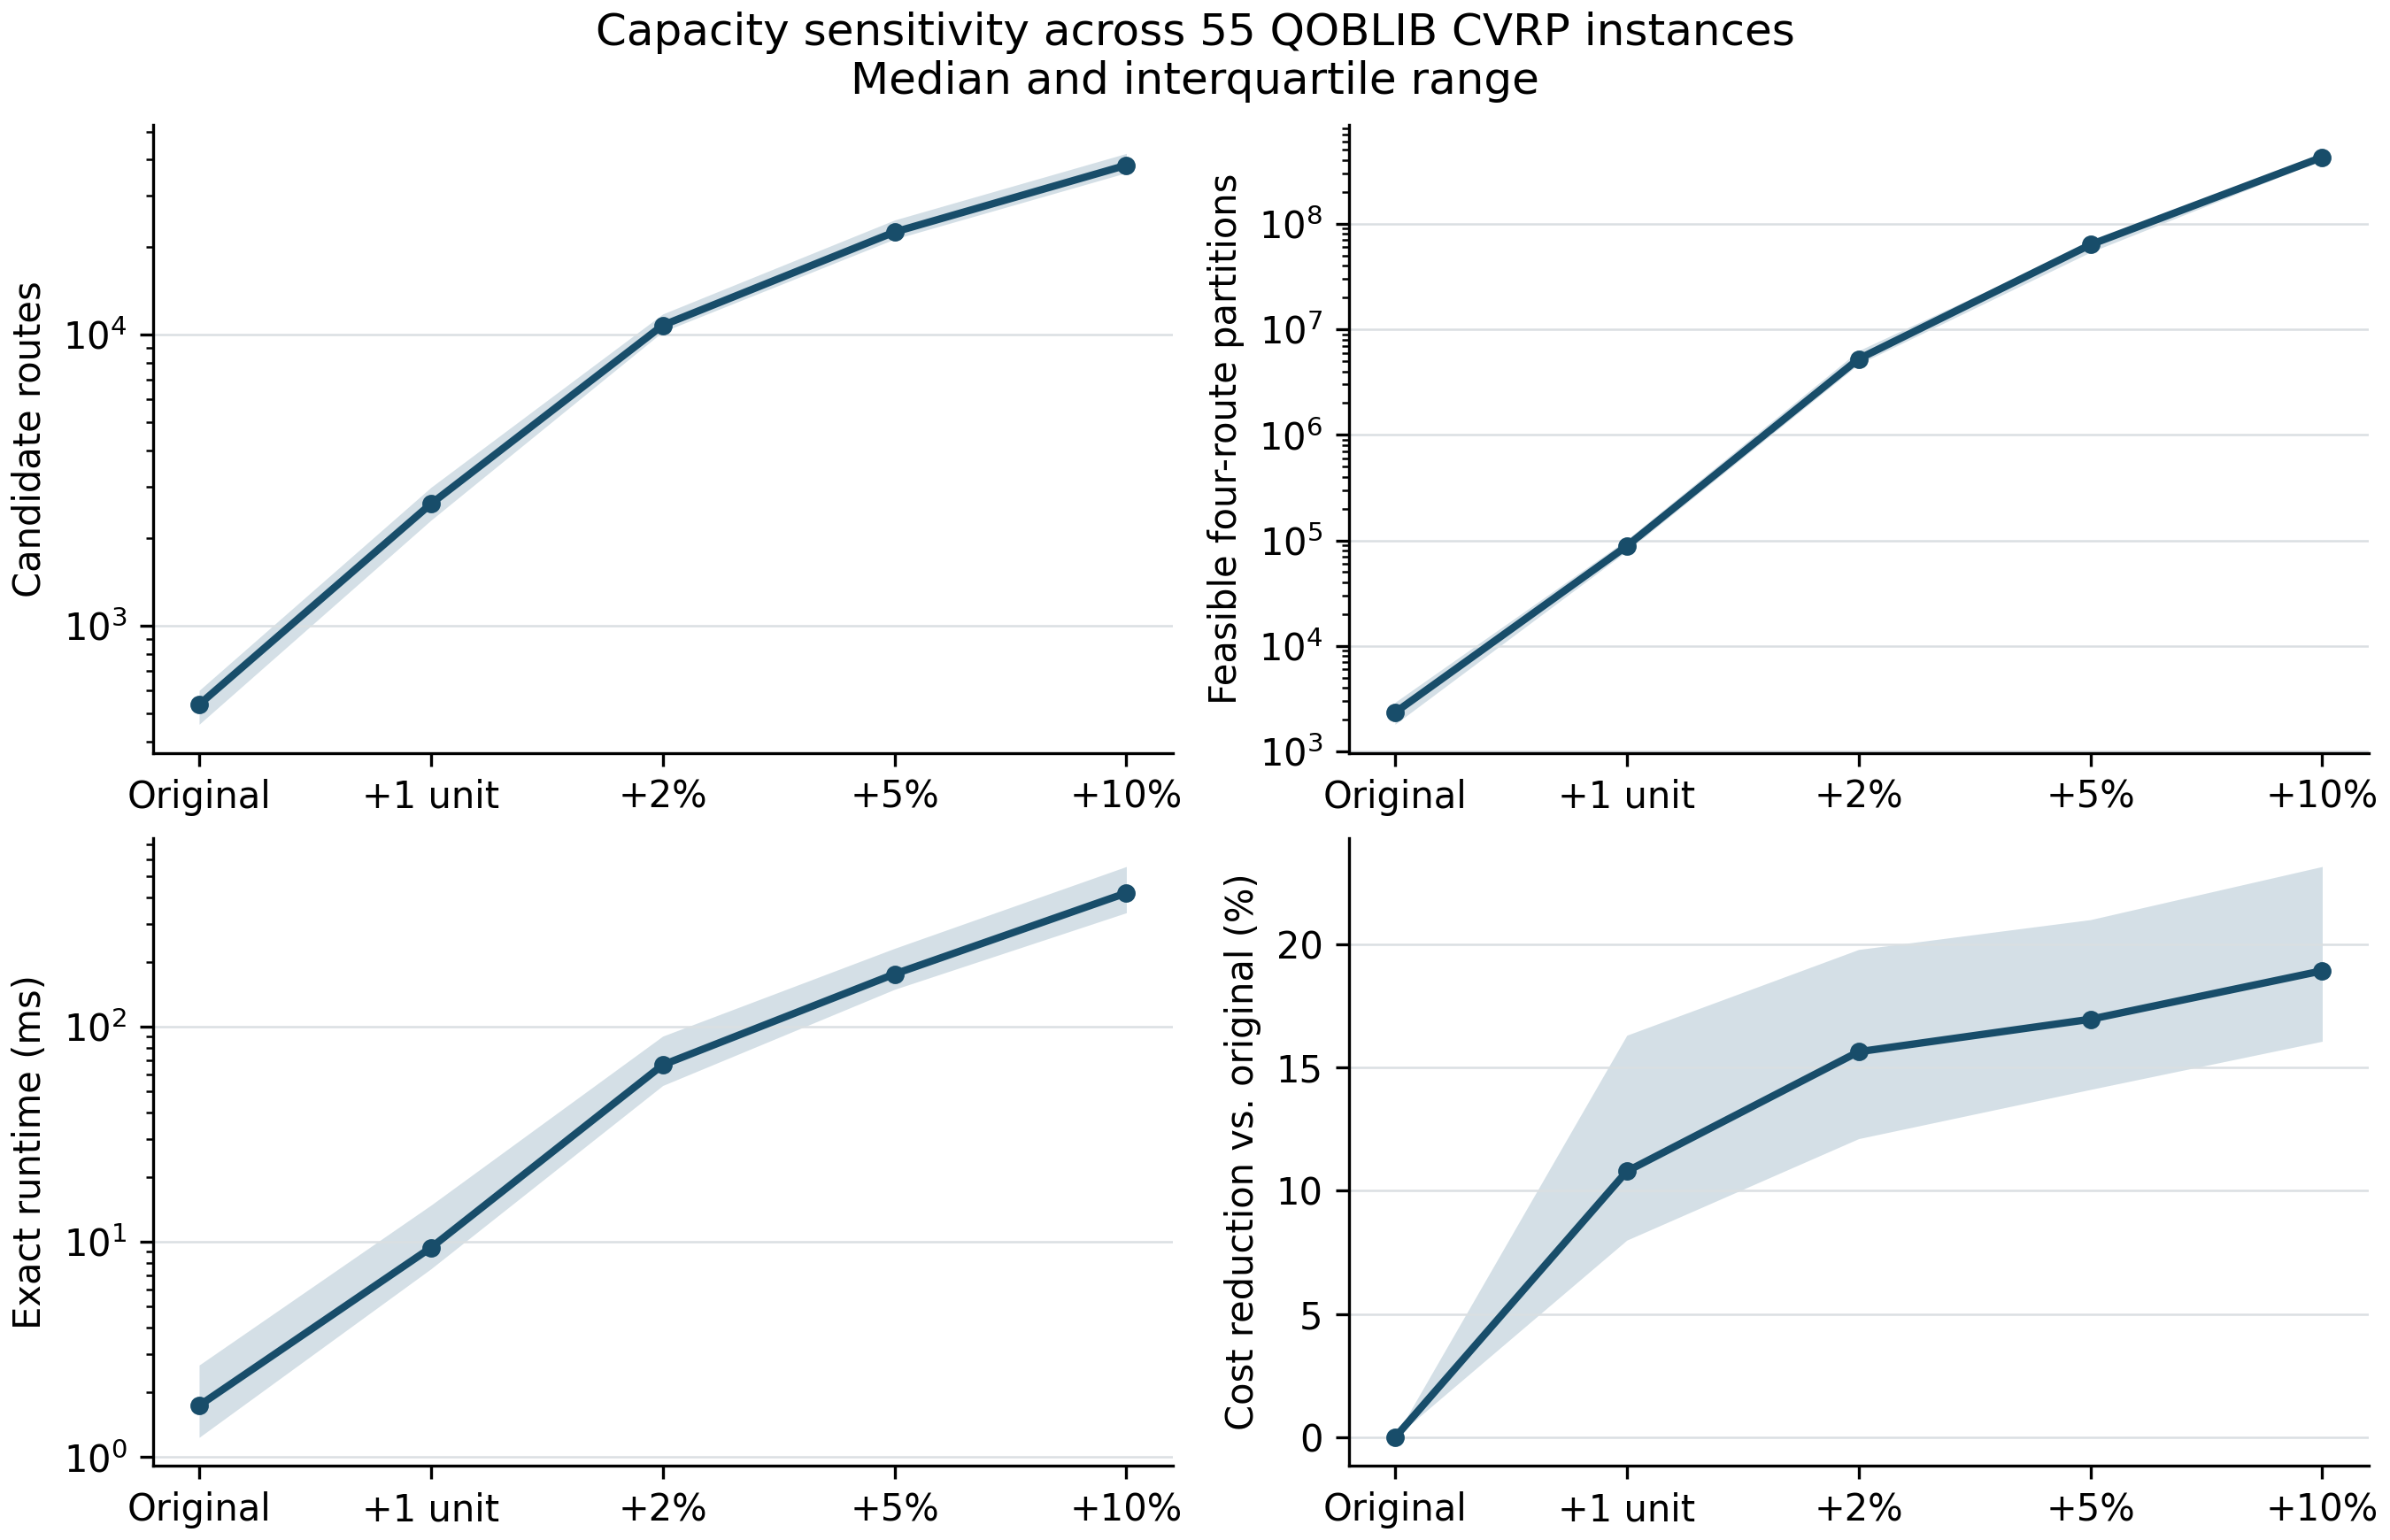
\includegraphics[width=\linewidth]{capacity-sensitivity.png}
\caption{Dispersion across the XSH suite along the capacity sweep. The center and band summarize the median and interquartile range at each setting. Each point along an instance's trajectory uses the same customer demands and coordinates.}\label{fig:sweep}
\end{figure}
\section{Full-parent load profiles}
\begin{table}[htbp]\centering
\caption{Full X parents at file capacity and the named fleet size. Discarded sets are exact integer differences. Retained percentages near 100 are rounded. No full-parent tours were priced.}\label{tab:parents}
\begin{tabular}{lrrrrr}\toprule
Parent & $C$ & $\Delta$ & $L(C)$ & Discarded sets & Retained (\%)\\\midrule
X-n101-k25 &206&3&203&6,033,103,589&21.4891\\
X-n106-k14 &600&536&64&32&100.0000\\
X-n110-k13 &66&42&24&341,125&100.0000\\
X-n115-k10 &169&155&14&8,675,767&100.0000\\
X-n120-k6 &21&7&14&88,758,031,322,592,943&99.9999\\
X-n125-k30 &188&104&84&87,180,228&99.9960\\
X-n129-k18 &39&37&2&16&100.0000\\
X-n134-k13 &643&139&504&830,885,602,224,370&99.6174\\
X-n139-k10 &106&21&85&23,222,548,376,026,685&99.8716\\
X-n143-k7 &1190&855&335&1,618,730,974,437,591&100.0000\\\bottomrule
\end{tabular}
\end{table}
\section{Edge-model validation}
We further test a separate undirected edge formulation on selected perturbed instances. Customer vertices have degree two, the depot has degree eight, and a depot edge can be used twice to permit a singleton tour. For each detected customer component $U$ that lacks enough connections, add the rounded-capacity constraint
\begin{equation}
 \sum_{e\in\delta(U)}x_e\ \geq\ 2\lceil d(U)/C\rceil.
\end{equation}
An intermediate model relaxes the routing problem, so a valid lower bound survives a timeout. This test uses distances and demands directly and shares no priced columns with the enumerator.


\begin{table}[htbp]\centering
\caption{Edge-model validation at 5\% extra capacity. A dash denotes absence of a verified edge-model incumbent within the budget. Instance identifiers are XSH suffixes.}\label{tab:arc}
\begin{tabular}{rrrrrr}\toprule
Rank & ID & Exact cover & Edge incumbent & Lower bound & Gap (\%)\\\midrule
1&16&779&--&693&11.04\\
8&45&905&--&885&2.21\\
15&33&441&--&426&3.40\\
21&48&455&--&429&5.71\\
28&20&522&--&481&7.85\\
35&12&602&--&578&3.99\\
41&40&540&540&540&0.00\\
48&22&592&592&592&0.00\\
55&34&631&--&621&1.58\\\bottomrule
\end{tabular}
\end{table}

\section{Paired outcomes for the one-unit increase}
Table~\ref{tab:pairs1} gives the per-instance observations behind the one-unit comparison. $H_0,H_1$ denote feasible partition counts at $Q$ and $Q+1$. These counts apply also to every shuffle of the corresponding instance. The last two columns compare the original percentage reduction with the median of the 51 shuffle reductions. Each shuffle uses its own optimal baseline distance in the denominator. The XSH identifiers use the prefix XSH-n20-k4-. Data originate from the QOBLIB routing files (credited there to Queiroga and Uchoa), revision 55384509. External X inputs use the VROOM benchmark mirror, revision 0f5ee1e. Derived capacities and demand reassignments are experimental modifications.
\newcommand{\pairhead}{\toprule ID & $Q$ & $z(Q)$ & $z(Q+1)$ & $H_0$ & $H_1$ & Original (\%) & Shuffle (\%)\\\midrule}
\begingroup\footnotesize
\begin{longtable}{rrrrrrrr}
\caption{Original and shuffled distance response, instances 01--55.}\label{tab:pairs1}\\
\pairhead\endfirsthead
\multicolumn{8}{c}{\tablename~\thetable\ (continued)}\\
\pairhead\endhead
\bottomrule\endfoot
\input pairs-1.tex \input pairs-2.tex
\end{longtable}
\endgroup
\section{Six-vehicle cohorts}
One hybrid uses 24 sites and one depot from each listed X parent. The three columns report optimal travel distance when four additional units are distributed as evenly as possible, as three plus one, or adaptively for the observed demands. The second cohort contains 20 parents held out from the initial ten; the 20 were chosen by rank in the pinned repository before computing their costs.
\begingroup\small
\begin{longtable}{llrrr}
\caption{Six-vehicle optimal distances, by source geometry and evaluation cohort.}\\
\toprule Cohort & Source geometry & Even & Three plus one & Adaptive\\\midrule\endfirsthead
\toprule Cohort & Source geometry & Even & Three plus one & Adaptive\\\midrule\endhead
\bottomrule\endfoot
Initial & X-n101-k25 & 8940 & 8847 & 8843 \\
Initial & X-n106-k14 & 12458 & 12340 & 12340 \\
Initial & X-n110-k13 & 6941 & 6818 & 6752 \\
Initial & X-n115-k10 & 7129 & 7031 & 6986 \\
Initial & X-n120-k6 & 12371 & 11993 & 11993 \\
Initial & X-n125-k30 & 12511 & 12418 & 12418 \\
Initial & X-n129-k18 & 11579 & 11469 & 11298 \\
Initial & X-n134-k13 & 5980 & 5980 & 5895 \\
Initial & X-n139-k10 & 8050 & 7954 & 7954 \\
Initial & X-n143-k7 & 12591 & 12284 & 12131 \\
New & X-n148-k46 & 7540 & 7485 & 7485 \\
New & X-n172-k51 & 7566 & 7372 & 7372 \\
New & X-n190-k8 & 11721 & 11587 & 11587 \\
New & X-n214-k11 & 5161 & 5136 & 5131 \\
New & X-n233-k16 & 7857 & 7740 & 7674 \\
New & X-n261-k13 & 12315 & 12184 & 12173 \\
New & X-n280-k17 & 12596 & 12375 & 12254 \\
New & X-n303-k21 & 6786 & 6685 & 6585 \\
New & X-n322-k28 & 8566 & 8368 & 8368 \\
New & X-n351-k40 & 4692 & 4625 & 4625 \\
New & X-n384-k52 & 9468 & 9363 & 9265 \\
New & X-n429-k61 & 8407 & 7839 & 7839 \\
New & X-n469-k138 & 12471 & 12032 & 12032 \\
New & X-n536-k96 & 7569 & 7650 & 7516 \\
New & X-n586-k159 & 9478 & 9261 & 9261 \\
New & X-n655-k131 & 6001 & 5920 & 5914 \\
New & X-n733-k159 & 8385 & 8205 & 8205 \\
New & X-n819-k171 & 7827 & 7737 & 7737 \\
New & X-n895-k37 & 10487 & 10216 & 10216 \\
New & X-n1001-k43 & 11264 & 11264 & 11264 \\
\end{longtable}\endgroup
\section{Filtering before pricing yields diminishing returns}
At the original capacity the paired median reduction in candidates is $51.44\times$ and the median pricing speedup is $25.72\times$. Table~\ref{tab:ablation} follows the same mechanism away from equality. With one extra unit the early filter discards about nine of every ten capacity-feasible sets on the median instance. All 55 cases run faster overall. At 5\% extra capacity it still reduces the median candidate pool by a factor of 1.51. The improvement in total time is smaller and its interquartile range crosses parity. All 165 early/late pairs agree on the four deterministic outputs.

\begin{table}[tb]\centering
\caption{Dedicated XSH ablation. Factors divide late by early measurements within each instance. The last column counts instances with strictly shorter total time under early filtering.}\label{tab:ablation}
\begin{tabular}{lrrrrr}\toprule
Increase & Candidate factor & Pricing factor & Total factor & Total IQR & Faster\\\midrule
1 unit &10.49&6.21&4.45&4.02--4.73&55/55\\
2\% &2.76&1.92&1.34&1.24--1.43&52/55\\
5\% &1.51&1.22&1.04&0.99--1.14&38/55\\\bottomrule
\end{tabular}
\end{table}

Two mechanisms help interpret the gap between columns. First, a discarded low-load subset can be cheaper to price than a retained subset with many customers. Second, both versions still combine surviving sets and solve the same cover problem. At 5\% extra capacity the sweep measures median early pricing time of 44.24 ms and median coverage time of 130.88 ms. Even a substantial change to pricing would affect only a portion of the total. These stage times describe this implementation and do not estimate the performance of a general-purpose CVRP solver.

\section{External samples and full-parent load profiles}
\paragraph{External timing and full-parent counts.}
For each of the ten smallest CVRPLIB-X parents, we shuffled customer IDs (seed 20261121) and took two disjoint 20-customer samples, retaining the original depot, coordinates and demands. We assigned demands in descending order to the lightest of four vehicles. The largest resulting load sets a feasible base capacity. We tested the same three increases as in the XSH ablation. After a slow pilot, we set a 12-second limit per mode for three repetitions and recorded completed pairs at each nominal level.

For the ten full parents, the load-count calculation uses the original demands, capacity and named fleet size. Together with XSH this gives 325 exact count pairs across five capacities. We verified all XSH counts against explicit enumeration.


Of the 60 external timing pairs, 54 completed both modes. The six excluded pairs are the two samples from X-n115-k10 at all three labels. For the remaining 18 pairs per label, total speedup medians were 1.055 at one unit, 1.031 at 2\% and 1.032 at 5\%. Early filtering was faster on 10, 11 and 15 pairs, respectively. All completed pairs agreed on objective, partition count, optimum multiplicity and second distinct objective. Both modes reconstructed feasible tours. Censoring a complete parent and constructing base capacities by packing limit the comparison. In particular we cannot assign the difference from XSH uniquely to initial slack. The data do show that matching the number of customers and vehicles alone fails to reproduce the XSH median timing gain.

\paragraph{Does the placement effect transfer?}
On the same 20 external samples, we also solved each original placement and seven seeded demand permutations at base capacity and one extra unit. We fixed this design and a five-second budget per solve before observing the external placement outcomes. Every completed solution was reconstructed, and candidate and partition counts agreed across completed placements at each capacity. Both solves finished for 152 of 160 assignment pairs. The eight incomplete pairs all came from one sample of X-n115-k10. We used parents with two complete samples so that each contributed equally. This left nine of the ten parents.

For each sample we subtracted the original percentage saving from the median saving over its seven shuffles. We averaged the two sample contrasts within each parent, then took the median over parents. The median contrast was zero. Four parent contrasts were negative, three were positive and two were zero. They ranged from $-1.51$ to $+1.91$ percentage points. The separately aggregated original and shuffled reductions were 1.08\% and 0.51\%. Subtracting these two medians would answer a different question. The original-placement premium observed on XSH did not recur as a median effect under this external design. Initial fleet slack, the demand distribution, and the relative size of one capacity unit all vary across these external samples.

Across the 325 demand-only profiles, each of 1,320 available enumeration records matched the independently computed exact candidate count. This tally includes timing repeats and covers 55 distinct XSH inputs. On the full X parents, the median retained fraction at base capacity exceeded 99.99\%; all ten discarded at least one set in exact arithmetic. On the original XSH suite the median fraction was only 1.94\%. Even on XSH it rose to 9.53\% at one extra unit, 36.22\% at 2\%, 66.10\% at 5\% and 89.12\% at 10\%. The calculation exposes the difference before any customer coordinates are read.



X-n101-k25 retains 1,651,308,169 of 7,684,411,758 sets in the load interval 203--206. X-n106-k14 discards only 32 of 336,289,328,182. Even a selective filter can leave billions of candidate sets to price.
\section{Computing partial-upgrade curves} For upgrade size $h$, let $z_b$ denote the minimum distance when at most $b$ of the four vehicles receive an upgrade.
We evaluated three cover implementations on all 55 XSH inputs at upgrade sizes $h=1$ and $h=2$. Direct enumeration visits each complete partition. An intermediate implementation chooses between scanning anchored submasks and scanning priced candidates to split the final remainder, and recomputes its three budget entries for each prefix. The cached implementation reuses these entries. All modes receive the same priced sets, and we rotated their order over three runs per mode per input and upgrade size. Timing covers the search and cache construction after parsing the priced sets; it excludes tour pricing, file transfer, reconstruction and cache teardown. All 110 configurations agreed across modes on exact-class costs and counts. Reconstructed witnesses attained the reported class costs and used the specified number of upgrades. The one-unit runs additionally reproduced all previously recorded budget optima and counts by exact class.

\begin{table}[tb]\centering
\caption{Route-combination time for an entire budget curve. Milliseconds are medians over instances after taking the within-instance median of three runs. Ratios are calculated within instance.}\label{tab:profiles}
\begin{tabular}{rrrrrr}\toprule
$h$ & Direct (ms) & Split (ms) & Cached (ms) & Direct/cached & Split/cached\\\midrule
1 & 9.49 & 10.09 & 3.89 & 2.42 & 2.61\\
2 & 50.58 & 50.54 & 12.96 & 4.02 & 3.93\\\bottomrule
\end{tabular}
\end{table}

Caching beat both alternatives in each of the 110 configurations. Relative to direct enumeration the interquartile range of the paired speedup was 2.22--2.58 at $h=1$ and 3.56--4.33 at $h=2$. Table~\ref{tab:profiles} also separates the effect of changing the split traversal from that of reusing its results. At $h=1$ switching traversal alone increased the median time slightly; reuse gave the main improvement. The timing comparison concerns implementations that return partition counts as well as optimal distances on these small instances.

\paragraph{Which budget choices does a flat fee miss?}
An upgrade budget $b>0$ is efficient if $z_b<z_{b-1}$. It is supported by a uniform fee if some $\lambda\geq0$ satisfies $z_b+\lambda b\leq z_a+\lambda a$ for every other budget $a$. We intersect these rational linear inequalities exactly, including ties. Counting the zero-upgrade endpoints, four of 150 efficient points at $h=1$ and three of 155 at $h=2$ were unsupported. Each occurred on a distinct instance within its setting. For instance~11 at $h=1$, choosing one upgrade over zero requires $908+\lambda\leq914$, or $\lambda\leq6$. Choosing it over two requires $908+\lambda\leq771+2\lambda$, or $\lambda\geq137$. A planner with a hard limit of one upgrade can nevertheless attain 908, strictly better than the baseline of 914. The budget profile makes this choice visible even when a sweep over all uniform fees would miss it.

\subsection{Budget profiles on the subset graph}
Let $Q$ be the base capacity and $t(S)$ the shortest depot tour through customer set $S$. Consider an upgrade of $h$ units per selected vehicle. Price each customer set once at capacity $Q+h$, and label it $e(S)=1$ if its load exceeds $Q$ and zero otherwise. A state $(R,t)$ comprises the remaining customer set and the number of routes still needed. An edge removes a priced subset $S\subseteq R$ containing the smallest remaining customer. Its distance is $t(S)$ and its upgrade label is $e(S)$. Let $F(R,t,j)$ be the minimum distance serving $R$ with $t$ routes of which exactly $j$ require an upgrade. The recurrence is
\[
 F(R,t,j)=\min_{S}\left\{t(S)+F(R\setminus S,t-1,j-e(S))\right\}.
\]
The empty state with zero routes and upgrades has distance zero. Infeasible entries have infinite cost. The count recurrence sums the child counts over the same edges, starting with one empty cover. The anchor orders each partition uniquely, and both edge quantities add over disjoint routes. Induction on $t$ therefore establishes both recurrences. Prefix minima over the root cost vector give all budget optima $z_b$.

For four vehicles we enumerate the first two anchored choices. For each remaining mask we compute three entries, one for each possible upgrade count on its final two routes. Each entry stores a count, a minimum cost and a witness split. Reusing the three entries on a repeated mask preserves how many covers each prefix represents. Keeping only its cheapest split would lose alternatives that use fewer upgrades. If $R$ occurs $m_R$ times and has $s_R$ candidate splits to test, reuse replaces $m_R s_R$ split tests with $s_R$ tests and $m_R$ constant-size merges. The cache occupies three entries per distinct two-route remainder reached. This is a budget-aware extension of the scalar remainder calculation; its benefit depends on how many masks recur.

\section{Counting candidate loads} Let $d_i$ denote customer demand, $C$ vehicle capacity and $L(C)$ the fleet-implied minimum feasible route load.
Let $a_s$ be the coefficient of $x^s$ in $\prod_{i\in N}(1+x^{d_i})$. Choosing the constant or nonconstant term for each customer gives a bijection between subsets and terms of the expanded product. With positive demands, the fraction of capacity-feasible nonempty customer sets retained by early filtering is exactly
\begin{equation}\label{eq:count}
 r(C)=\frac{\sum_{s=L(C)}^C a_s}{\sum_{s=1}^C a_s}.
\end{equation}
Initialize $a_0=1$ and all other entries to zero. For each demand $d$, update $a_s\gets a_s+a_{s-d}$ in descending load order. Computing all coefficients through $C_{\max}$ takes $O(nC_{\max})$ arbitrary-precision additions and $O(C_{\max})$ entries. Counting partitions also requires disjointness information.

\section{Distributions across the 55 XSH instances}
\begin{figure}[htbp]\centering
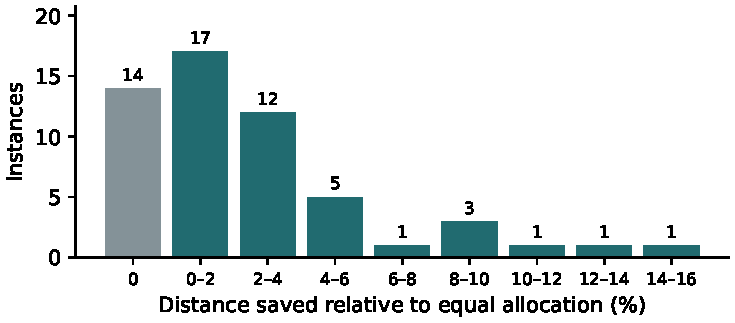
\includegraphics[width=.92\linewidth]{allocation-histogram.pdf}
\caption{Distance saved by the adaptive four-unit allocation relative to an equal allocation. Zero denotes a tie. Each positive interval excludes its lower endpoint and includes its upper endpoint.}
\end{figure}
\begin{figure}[htbp]\centering
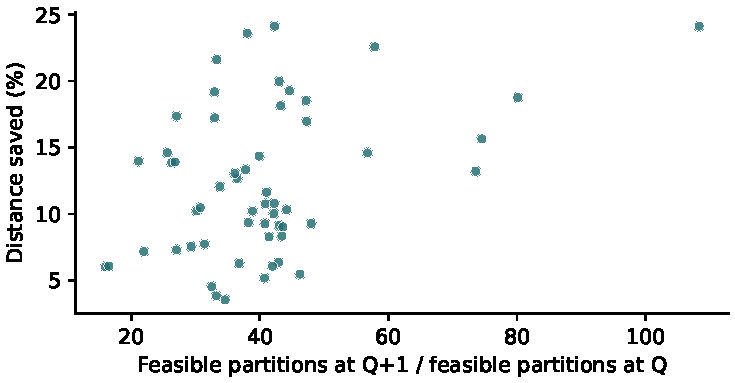
\includegraphics[width=.92\linewidth]{partition-growth.pdf}
\caption{Effect of adding one unit to each vehicle. Each point pairs partition growth and optimal-distance reduction on the same XSH instance. Both quantities use its original capacity as the baseline.}
\end{figure}
\end{document}
